\documentclass{article}
\usepackage{amsmath,amssymb}
\usepackage{graphicx}
\usepackage{xcolor}
\usepackage{listings}
\usepackage{fancyhdr}



\pagestyle{fancy}
\fancyhf{}

\rhead{\leftmark}
\fancyfoot[LE,RO]{\thepage}


\renewcommand{\baselinestretch}{1.2}
\setlength{\parskip}{1em}
\definecolor{codegreen}{rgb}{0,0.6,0}
\definecolor{codegray}{rgb}{0.5,0.5,0.5}
\definecolor{codepurple}{rgb}{0.58,0,0.82}
\definecolor{backcolour}{rgb}{0.95,0.95,0.92}

\usepackage{hyperref}
\hypersetup{
    colorlinks,
    citecolor=black,
    filecolor=black,
    linkcolor=black,
    urlcolor=black
}


\lstdefinestyle{mystyle}{
    backgroundcolor=\color{backcolour},   
    commentstyle=\color{codegreen},
    keywordstyle=\color{magenta},
    numberstyle=\tiny\color{codegray},
    basicstyle=\ttfamily\footnotesize,
    breakatwhitespace=false,         
    breaklines=true,                 
    captionpos=b,                    
    keepspaces=true,                 
    numbers=left,                    
    numbersep=5pt,                  
    showspaces=false,                
    showstringspaces=false,
    showtabs=false,                  
    tabsize=2
}

\lstset{style=mystyle}

\begin{document}

\newpage{}
\tableofcontents
\newpage{}

\newpage
\section{Stable Maching problema}

\subsection{Algoritmo Gale-Shapley}
Este algoritmo al terminar de ejecutarse se encuentra un matching prefecto si:
\begin{itemize}
    \item Si existen \(n\) solicitantes con diferentes preferencias.
    \item Si existen \(n\) requeridos con diferentes preferencias.
\end{itemize}
Eligiendo las estructuras correctamente se puede plantear en \(O(n)\).

\begin{lstlisting}[language=Python, caption=Algoritmo de Gale-Shapley]
    Inicialmente M=Vacio
    
    Mientras existe un solicitante sin pareja que no aun se haya postulado a todas las parejas
    
        Sea s un solicitante sin pareja
        Sea r el requerido de su mayor preferencia al que no le
                    solicito previamente
            
        if r esta desocupado
            M = M U (s,r)
            s esta ocupado
        else
            Sea s' tal que (s', r) pertenece a M

            si r prefiere a s sobres s'
                M = M - {(s', r)} U (s,r)
                s esta ocupado
                s' esta libre
    Retornar M
    
\end{lstlisting}    

\newpage
\subsection{Alternativas}
\subsubsection{Diferentes cantidades de oferentes que requeridos}

Dado n oferentes y m requeridos, con \(m <> n\), no se puede encontrar un matching stable. 

Entonces, tenemos que redefinir el concepto de estable. Una pareja (s,r) es \textbf{estable} si:
\begin{itemize}
    \item No existe requerido r' sin pareja al que s prefiera a su actual pareja.
    \item No existe un requerido r' en pareja, tal que s y r' se prefieran sobre sus respectivas parejas.
    \item No existe solicitante s' sin pareja al que r prefiera a su actual pareja.
    \item No existe un solicitante s' en pareja tal que r y s' se prefieran sobre sus respectivas parejas.
\end{itemize}    


Por lo tanto un matching es estable si:
\begin{itemize}
    \item No tienen parejas inestables bajo la condicion anterior.
    \item Que no queden requeridos y solicitantes sin pareja.
\end{itemize}

Soluciones para ajustar al modelo de Gale-Shapley:
\begin{enumerate}
    \item Inventar \(|n-m|\) elementos ficticios
    \begin{itemize}
        \item Los elementos ficticios se pondran en las listas de preferencias con menos elementos.
        \item Estos elementos ficticios se agregan al final y deben ser los menos preferidos.
        \item Luego ejecutar Gale-Shapley
        \item Por ultimo, eliminar las parejas con elementos ficticios. Estos seran los requeridos que quedan sin pareja.
    \end{itemize}
    \item Adecuar el Algoritmo
    \begin{itemize}
        \item Si hay mas \textbf{solicitantes} que requeridos, quitar de la \textit{lista de solicitantes} sin parejas a aquellos que agotaron sus propuestas.
        \item Si hay mas \textbf{requeridos} que solicitantes, quitar de la \textit{lista de parejas} a aquellas donde el requerido quedo sin pareja.
    \end{itemize}
\end{enumerate}

\newpage
\subsubsection{Preferencias incompletas}
Las listas de preferencias de los oferentes y los requeridos son un subset de las contrapartes.

Son parejas \textbf{aceptables} de un elemento a aquellas contrapartes que figuran en su lista de preferencias.

Una pareja (s,r) es \textbf{estable} si:
\begin{itemize}
    \item Son \textit{aceptables} entre ellos.
    \item No existe requerido \textit{aceptable} r' sin pareja al que s prefiera a su actual pareja.
    \item No existe un requerido \textit{aceptable} r' en pareja, tal que s y r' se prefieran sobre sus respectivas parejas.
    \item No existe solicitante \textit{aceptable} s' sin pareja al que r prefiera a su actual pareja.
    \item No existe un solicitante \textit{aceptable} s' en pareja tal que r y s' se prefieran sobre sus respectivas parejas.
\end{itemize}

\begin{quote}
    \textbf{Un matching es estable si no tiene parejas inestables bajo la condicion anterios.}
\end{quote}

\begin{lstlisting}[language=Python, caption=Algoritmo para parejas incompletas]
Inicialmente M=Vacio

#Iterea mientras no haya acotado su sublista de preferencias
Mientras existe un solicitante sin pareja
                'que no aun se haya postulado a todas las parejas' 

    Sea s un solicitante sin pareja
    Sea r el requerido de su mayor preferencia al que no le
                solicito previamente
    
    # se condiera si es aceptable
    if r considera 'aceptable' a s

        if r esta desocupado
            M = M U (s,r)
            s esta ocupado
        else
            Sea s' tal que (s', r) pertenece a M
            si r prefiere a s sobres s'
                M = M - {(s', r)} U (s,r)
                s esta ocupado
                s' esta libre

# Retornar solo parejas aceptables
Retornar M

\end{lstlisting}    


\subsubsection{Preferencias con empates}


\textbf{INDIFERENCIA Y PREFERENCIA ESTRICTA}

\begin{enumerate}
    \item X es \textbf{indiferente} a "y" y a "z" si en su lista de preferencias estan el la misma posicion.
    \item X es \textbf{prefefiere estrictamente} a "y" sobre "z" si en su lista de preferencias no le son indiferentes y 
          "y" se encuentra antes que "z" en la misma.
\end{enumerate}

\noindent
\textbf{ESTABILIDAD DEBIL}
\newline Una pareja (s,r) es debilmente estable si no existe una pareja (s' y r') talque:
\begin{itemize}
    \item s prefiere estrictamente a r' sobre r \textit{(pareja actual de s)}
    \item r' prefiere estrictamente a s sobre s' \textit{(pareja actual de r')}
\end{itemize}



\begin{lstlisting}[language=Python, caption=Algoritmo para parejas incompletas]
    Inicialmente M=Vacio
    
    #Iterea mientras no haya acotado su sublista de preferencias
    Mientras existe un solicitante sin pareja
                    'que no aun se haya postulado a todas las parejas' 
    
        Sea s un solicitante sin pareja
        Sea r el requerido de su mayor preferencia al que no le
                    solicito previamente
            
        if r esta desocupado
            M = M U (s,r)
            s esta ocupado
        else
            Sea s' tal que (s', r) pertenece a M

            # prefiere estrictamente
            si r prefiere estrictamente a s sobres s'
                M = M - {(s', r)} U (s,r)
                s esta ocupado
                s' esta libre
    
    Retornar M
    
\end{lstlisting}    
\begin{quote}
    En caso de que sea empate, se mantendra con su pareja actual.
\end{quote}

\noindent
\textbf{ESTABILIDAD FUERTE}
\newline Una pareja (s,r) es debilmente estable si no existe una pareja (s' y r') talque:
\begin{itemize}
    \item s prefiere estrictamente o le es indiferente a r' sobre r \textit{(pareja actual de s)}
    \item r' prefiere estrictamente o le es indiferente a s sobre s' \textit{(pareja actual de r')}
\end{itemize}
Puede no existir un matching perfecto.

\begin{lstlisting}[language=Python, caption=Algoritmo para parejas super estables]
    Inicialmente M=Vacio
    
    Mientras existe un solicitante sin pareja y no exista solicitante que agoto sus parejas
    
        Sea s un solicitante sin pareja
        Sea r el requerido de su mayor preferencia al que pueda proponer
        Por cada sucesor s' a s en la lista de preferencias de r
            if (s',r) pertence a M
                M = M - {(s',r)}
                s' esta libre
            quitar s' de la lista de preferencias de r
            quitar r de la lista de preferncias de s'

        Por cada requerido r' que tiene multiples parejas
            Por cada pareja s' en pareja con r' 
                M = M - {(s',r')}
                quitar s' de la lista de preferencias de r'
                quitar r' de la lista de preferencias de s'

    if estan todos en pareja
        Retornar M
    else
        No existe ningun matching super estable
\end{lstlisting}    
\begin{quote}
    En caso de que sea empate, se mantendra con su pareja actual.
\end{quote}

\newpage
\subsubsection{Agrupacion de 1 a muchos}
El solicitante puede tener varios cupos por lo tanto:
\begin{itemize}
    \item Exiten \(m\) requeridos, donde un requerido puede estar unicamente con 1 pareja.
    \item Exiten \(n\) solicitantes, donde cada solicitante puede tener \(c\) cupos para armar parejas.
\end{itemize}

Existe un matching estable si la cantidad de requeridos es igual a la cantidad de solicitantes por la cantidad de cupos.

\begin{equation} \label{eu_eqn}
    m=n*c
\end{equation}

No cambia la definición de Gale Shampey para \textbf{matching estable}

\begin{lstlisting}[language=Python, caption=Algoritmo de solicitantes con cupos]
    Inicialmente M=Vacio
    
    Mientras exista un solicitante con cupo disponible
    
        Sea s un solicitante sin pareja
        Sea r el requerido de su mayor preferencia al que no le
                    solicito previamente
            
        if r esta desocupado
            M = M U (s,r)
            s decremente su disponibilidad de parejas
        else
            Sea s' tal que (s', r) pertenece a M

            si r prefiere a s sobres s'
                M = M - {(s', r)} U (s,r)
                s decremente su disponibilidad de parejas
                s' incrementa su disponibilidad de parejas
    Retornar M
    
\end{lstlisting}    
\begin{quote}
    \textbf{La complejidad algoritmica no se modifica porque solo se agrega un contador.}
\end{quote}

\newpage
\subsubsection{Agrupacion de muchos a 1}
El requerido puede tener varios cupos por lo tanto:
\begin{itemize}
    \item Exiten \(m\) requeridos, donde cada solicitante puede tener \(z\) cupos para armar parejas.
    \item Exiten \(n\) solicitantes, donde un requerido puede estar unicamente con 1 pareja.
\end{itemize}

Existe un matching estable si la cantidad de solicitantes es igual a la cantidad de requeridos por la cantidad de cupos.

\begin{equation} \label{eu_eqn}
    n=m*z
\end{equation}

No cambia la definición de Gale Shampey para \textbf{matching estable}

\begin{lstlisting}[language=Python, caption=Algoritmo de requeridos con cupos]
    Inicialmente M=Vacio
    
    Mientras exista un solicitante con cupo disponible
    
        Sea s un solicitante sin pareja
        Sea r el requerido de su mayor preferencia al que no le
                    solicito previamente
            
        if r tiene cupo 
            M = M U (s,r)
            s esta ocupado
            r decrementa su disponibilidad de parejas
        else
            Sea s' tal que (s', r) pertenece a M y 
                    s' es el menos preferidos de las parejas r

            si r prefiere a s sobres s'
                M = M - {(s', r)} U (s,r)
                s esta ocupado
                s' esta libre
    Retornar M
    
\end{lstlisting}    
\begin{quote}
    \textbf{La complejidad algoritmica si se modifica.}
\end{quote}
Para conocer el solicitante de menor preferencia podemos utilizar un heap de minimos. Como el cupo es de z, la complejidad algoritmica para actualizar el heap es \(log (z)\).

\newpage
\subsubsection{Agrupacion de y a x}
\begin{itemize}
    \item Exiten \(n\) solicitantes, donde cada solicitante puede tener \(c\) cupos para armar parejas.
    \item Exiten \(m\) requeridos, donde cada requerido puede tener \(z\) cupos para armar parejas.
\end{itemize}


Existe un matching estable si:

\begin{equation} \label{eu_eqn}
    n*c=m*z
\end{equation}


No cambia la definición de Gale Shampey para \textbf{matching estable}
\newline
Para implementar se requieren las siguientes estructuras:
\begin{itemize}
    \item Un heap de minimos para los requeridos.
    \item Un contador de cupos para los solicitantes.
\end{itemize}

\begin{quote}
    \textbf{La complejidad algoritmica es igual a la de los requeridos con cupos}
\end{quote}

\newpage
\subsubsection{Conjuntos no bipartios - Stable Roommate Problem}
Pendiente

\newpage
\section{Analisis amortizado}

\subsubsection{Metodo de agregacion}
\subsubsection{Metodo del banquero}
\subsubsection{Metodo del potencial}

\newpage
\subsubsection{Heap binomial y fibonacci}
Revisar capitulo 19 del Corven.
\newline
Para el \textbf{heap binomial} se utilizan bosques de arboles binarios. Existe un proceso donde se van ordenando los arboles.

Al insertar, se parece al ejemplo de contador binario y la amortizacion es O(1)
\newline
Decrementar en un log binomial, es log(n) porque no es posible amortizar
\newline 
Eliminar el minimo, es el el peor caso es log(n)

Para el \textbf{heap fibonacci} ...

\section{Algoritmos Greedy}

Utiliza heurisica de seleccion para encontrar una solución global optima despues de muchos pasos.

\subsection{Mochila fraccionaria}

Dado un contener de capacidad W, y un conjunto de elementos n fraccionables de valor \(v_i\) y peso \(w_i\)

El objetivo es seleccionar un subconjunto de elemento o fracciones de ellos de modo de maximizar el valor almacenado y sin superar la capacidad de la mochila.

La complejidad es \(O(nlog(n))\)

\newpage
\subsection{Cambio de moneda}

Es una solución es conocido como solución de cajero. Contamos con un conjunto de diferentes monedas de diferentes denominación sin restricción de cantidad.

\[
    \$=(C_1,C_2,C_3,\cdots,C_n)  
\]

El objetivo es entregar la menor cantidad posible de monedas como cambio.

Tiene una complejidad de \(O(n)\).

El sistema \(\$\) se conoce como \textbf{canonico} a aquel en el que para todo x, \(greedy(\$,x)=optimo(\$,x)\).

Para saber si una base es canonica:
\begin{enumerate}
    \item Basta con buscar un contraejemplo. Estaria entre la 3ra denomininacion y la suma de las ultimas dos doniminaciones.
    \item Utilizar un algoritmo Polinimico para determinar si es un sistema canonico.
\end{enumerate}

Si el problema no es greddy, se puede construir un algoritmo utilizando programación dinamica.


\newpage
\subsection{Interval Scheduling: Algoritmo de Greedy Stay Ahead}

Tenemos un conjunto de requests \(\{1,2,..,n\}\); el request \(i^{th}\) corresponde a un intervalo de tiempo que comienza al instante \(s(i)\) y finaliza al instante \(f(i)\).
Diremos que un subconjunto de requests es compatible si no hay dos de ellos que al mismo tiempo se superponen, y nuestro objetivo es aceptar un subconjunto compatible tan grande como sea posible. El conjunto compatible con mayor tamaño sera el \textbf{óptimo}.

La idea básica en un algoritmo greedy para interval scheduling es usar una simple regla para seleccionar el primer request \(i_1\). Una vez que el request \(i_1\) aceptado, rechazamos todos los request que no son compatibles con \(i_1\). Luego seleccionamos el siguiente request \(i_2\), y volvemos a rechazar todos lo request que no son compatibles con \(i_2\). 
Continuamos de esta manera hasta que nos quedemos sin requests. El desafio en diseñar un buen algoritmo greedy esta en decidir que regla usar para la selección.

Pueden probar con varias reglas, pero las mas optimo es la siguiente idea: Aceptaremos el request que termina primero, o sea el request para el cual tiene el menor \(f(i)\) posible. 
Asi nos aseguramos que nuestros recursos se liberen tan pronto como sea posible mientras satisfacemos un request. De esta manera podemos maximizar el tiempo restante para satisfacer otro request.

Para escribir el pseudo código, utilizaremos \(R\) para denotar al conjunto de request que aún no estan aceptados ni rechazados, y usaremos \(A\) para denotar al conjunto de los request aceptados.

\begin{lstlisting}[language=Python, caption=Algoritmo de greedy para Interval Scheduling]
Inicialmente R contiene todos los requests, y A es un conjunto vacio.

Mientras R no esta vacio

    Seleccionar un request i de R que tenga el instante de finalizacion mas chico.
    Agregar el registro i a A
    Eliminar todos los request de R que no sean compatibles con el request i    

Fin mientras

Retornar el conjunto A como el conjunto de los request aceptados.

\end{lstlisting}    


\begin{figure}[h!]
    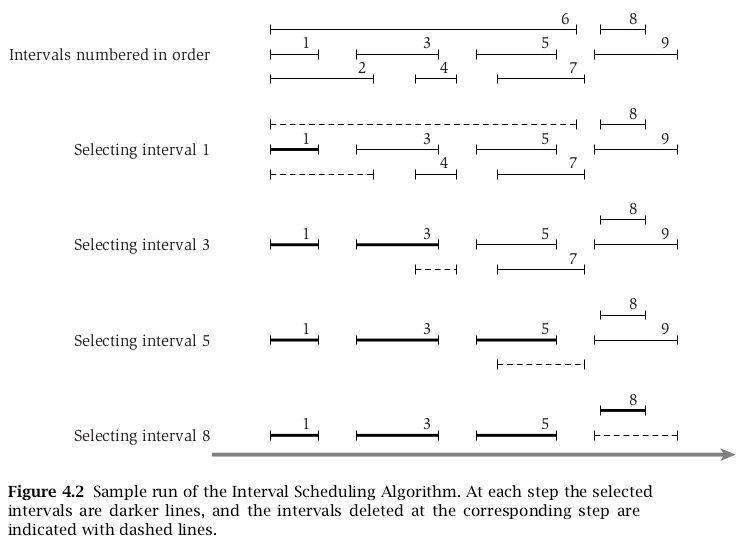
\includegraphics[width=\linewidth]{imagenes/intervalos-compatibles.png}
\end{figure}

\begin{quote}
    De forma inmediata podemos decir que el conjunto retornado tiene request compatibles.
\end{quote}

Lo que necesitamos es demostrar que la solución es optima. Definimos a \(O\), un conjunto de intervalos optimos. 
Luego, vamos a mostrar que \(|A| = |O|\), o sea que el conjunto \(A\) tiene la misma cantidad de intervalos que \(O\), y por lo tanto, \(A\) tambien es una solución optima.

Para la prueba introduciremos la siguiente notación:
\begin{itemize}
    \item Dado \(\{i_1,...,i_k\}\) el conjunto de request en \(A\) en orden que fueron agregados a \(A\). Notar que \(|A|=k\).
    \item Dado \(\{j_1,...,j_m\}\) el conjunto de request en \(O\) ordenos de izquierda a derecha. Notar que \(|O|=m\).
\end{itemize}
El objetivo es probar que \(k=m\).

La manera en que el algoritmo de greedy se mantenga adelante(\textbf{stays ahead}) es que cada uno de sus intervalos finalice al menos tan pronto como lo haga el correspondiente intervalo en el conjunto \(O\).

\begin{figure}[h!]
    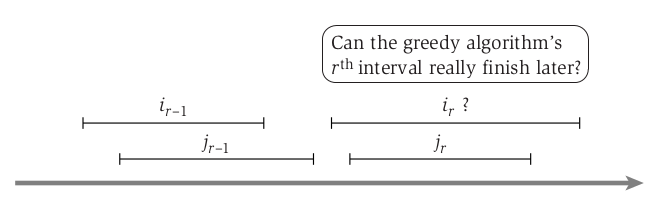
\includegraphics[width=\linewidth]{imagenes/demo-greedy-intervalos.png}
\end{figure}

\begin{quote}
    \textbf{(3.1) Para todos los indices \(r<k\) tenemos que \(f(i_r) \leq f(j_r)\)}
\end{quote}

\textbf{Demostración:}  Probaremos la sentencia anterior mediante el método inductivo. Para \(r=1\) la sentencia anterior es cierta, el algoritmo empieza seleccionando el request \(i_1\) con el menor tiempo de finalización.

Para el caso inductivo, o sea \(r>1\) asumiremos como nuestra hipotesis inductiva que la sentencia es verdadera para \(r-1\), y queremos probar que es tambien es lo es para \(r\). La hipotesis inductiva nos dice que asumamos verdadero que \(f(i_{r-1}) \leq f(j_{r-1})\). Queremos demostrar que \(f(i_{r}) \leq f(j_{r})\).

Dado que \(O\) consiste en intervalos compatibles, sabemos que \(f(j_{r-1}) \leq s(j_r)\). Combinando esto último con la hipotesis inductiva \(f(i_{r-1}) \leq f(j_{r-1})\), obtenemos \(f(i_{r-1}) \leq s(j_{r})\). Asi el intervalo \(j_r\) esta en conjunto \(R\) de los intervalos disponibles al mismo tiempo cuando el algoritmo de greedy selecciona \(i_r\).
El algoritmo de greedy selecciona el intervalo con el \textit{tiempo final mas chico} (\(i_{r}\)); y dado que intervalo \(j_{r}\) es uno de estos intervalos, tenemos que \(f(i_r) \leq f(j_r)\), completando asi el paso inductivo.

De esta forma demostramos que nuestro algoritmo se mantiene adelante del conjunto optimo \(O\). Ahora veremos porque esto implica optimalidad del conjunto \(A\) de algoritmo de greedy.

\begin{quote}
    \textbf{El algoritmo de greedy retorna un conjunto \(A\) óptimo.}
\end{quote}

\textbf{Demostración:} Para demostrarlo utilizaremos la contradicción. Si \(A\) no es optimo, entonces el conjunto \(O\) debe tener mas requests, o sea que tenemos \(m>k\) y aplicando 3.1, cuando r=k, 
obtenemos que \(f(i_k) \leq f(j_k)\). Dado que \(m>k\), existe un request \(j_{k+1}\) en \(O\). Este request empieza despues que el request \(j_k\) termina y por consiguiente despues de que el request \(i_k\) termine.
Entonces, despues de eliminar todos los requests que no son compatibles con los request \(i_1,...,i_k\), el conjunto de posibles requests R aún contiene el requests \(j_{k+1}\). 
Pero el algoritmo de greedy se detiene con el request \(i_k\) y este supuestamente se detiene porque \(R\) esta vacio, lo cual es una contradicción. 


\newpage
\subsection{Seam Carving - TODO}
Es un algoritmo para adecuar imagenes. Analiza imagenes recortando pixeles de menor importancia. Retira tantas vetas como sea necesario para llegar a un tamaño optimo.


\subsection{Caminimos Minimos - TODO}

Dado dos nodos, uno inicial \(s\) y otro final \(t\) el algoritmo encuentra el camino minimo que los une, tambien entre \(s\) y el resto de los nodos.

\subsection{Compresión de datos - TODO}

El algoritmo de greedy arma un arbol de "hufman" para armar un arbol optimo de prefijos.

\section{División y conquista}

\subsection{Teorema mestro - TODO}


\subsection{Mediana con datos separadas}




\newpage
\section{Programación dinamica}

\subsection{Cambio de monedas}

Contamos con un conjunto de monedas de diferente denominación sin restricción de cantidad. 
Representamos de esta manera \(\$=(c_1,c_2,....,c_n)\) y tenemos un importe \(x\) a dar. 
Concluimos que no existe un algoritmo satisfactorio de greedy para resolver este problema.

Si buscamos la solución por \textbf{fuerza bruta}, se puede armar un arbol de decisión. 
Por cada moneda posible, se genera un subproblema. 

\begin{figure}[h!]
    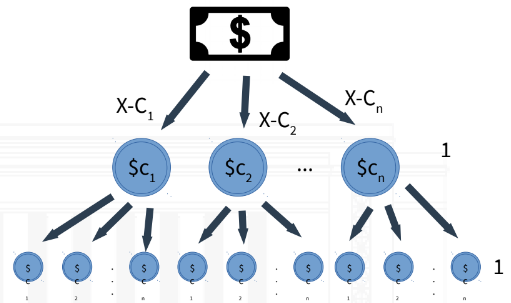
\includegraphics[width=\linewidth]{imagenes/dinamico-arbol-moneda.png}
\end{figure}

Entonces el camino a la hoja con menor profundidad es la menor cantidad de monedas a dar. Esto hace que la complejidad sea \(O(x^n)\).

Analizando el problema anteriores se pueden obtener algunas mejoras. 
Parte de los caminos del arbol son iguales. 
Hay distintas ramas con nodos que tienen el mismo resto, 
y por lo tanto se puede calcular solo una vez. 
Este caso de resto igual en varios nodos, lo llamaremos subproblemas.

\begin{figure}[h!]
    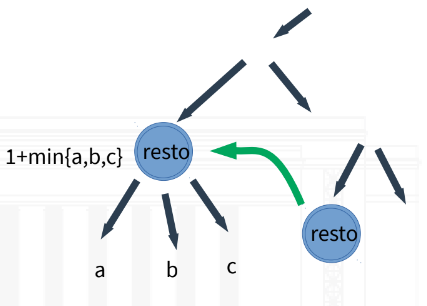
\includegraphics[scale=0.5]{imagenes/dinamico-moneda-subproblema.png}
\end{figure}

\newpage
\textbf{Subproblema}: Calcular el óptimo(OPT) del cambio \(x\) debe usar el mínimo entre los subproblemas \(X - C_j\) para \(j=1...n\).

Cada vez que paso por un subproblema se incremente en \(1\) para contar la cantidad de monedas a dar. 
Que seria: \(1+min\{subproblemas\}\).

Para la solución \textbf{recurrente}, podemos plantear:

    \[
        \left\{ \begin{array}{lcc}
            OPT(x) = 0 &   si  & x = 0 \\
            \\ OPT(x) = 1+min\{OPT(x-C_i)\} &  si & x > 0 \\
            \end{array}
        \right.
    \]

El resultado con el minimo cambio sera OPT(x) y para poder calcularlo, 
necesito calcular los \(x-1\) óptimos anterios. 
Para evitar el recalculo, si calculo el optimo de algun resto, 
lo almaceno para no volver a calcularlo de nuevo.
Ademas en cada subproblema debo analizar \(n\) comparaciones, lo cual impacta en la complejidad.

\noindent
\underline{SOLUCIÓN ITERATIVA}
\begin{lstlisting}[language=Python, caption=Solución iterativa]

OPT[0] = 0
Desde i=1 a X
    minimo = +infinito
    Desde j=1 a n
        resto = i - C[j]
        si resto > 0 y minimo > OPT[resto]
            minimo = OPT[resto]
    
    OPT[i] = 1 + minimo

Retornar OPT[X]
\end{lstlisting}

La complejidad es \(O(X*n)\) porque no solo depende de los diferentes tipos de monedas, tambien
depende del parametro de entrada \(X\). Se dice que es un algoritmo pseudo polinomial.

\noindent
\underline{RECONSTRUIR LAS ELECCIONES}

\begin{lstlisting}[language=Python, caption=Solución iterativa con reconstrucción]

OPT[0] = 0
elegida[0] = 0
Desde i=1 a X
    minimo = +infinito
    elegida[i] = 0
    Desde j=1 a n
        resto = i - C[j]
        si resto > 0 y minimo > OPT[resto]
            elegida[i] = j
            minimo = OPT[resto]
    
    OPT[i] = 1 + minimo

resto = x
Mientras resto > 0
    Imprimir C[elegida[resto]]
    resto = resto - C[elegida[resto]]

Imprimir OPT[x]

\end{lstlisting}

\newpage
\subsection{Problema de la Publicidad en la carretera}

Sea una carretera de longitud \(M\) km, un conjunto de \(n\) carteles publicitarios en el 
intevalo \([0,M]\), cada cartel \(i\) tiene una posición \(x_i\) y un valor de ganancia \(r_i\).
Entonces queremos seleccionar carteles para maximizar la ganancia. Como restriccción ningún cartel
puede estar a menos de 5 km de otro.

\begin{figure}[h!]
    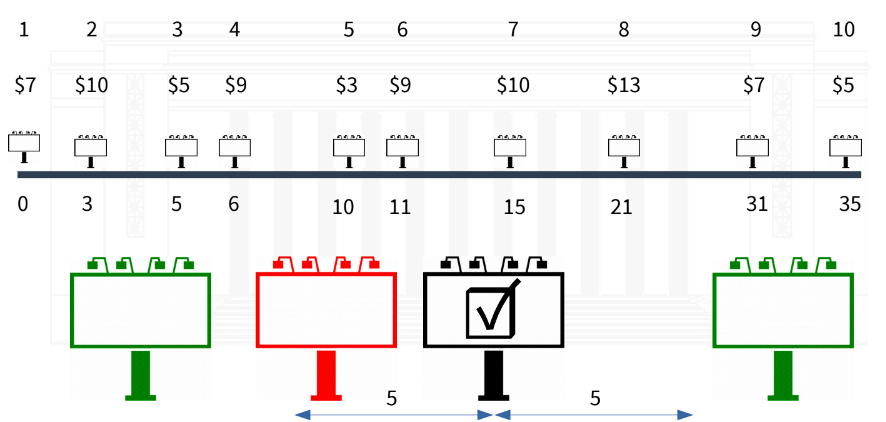
\includegraphics[scale=0.4]{imagenes/dinamico-ejemplo-ruta.png}
\end{figure}

Podemos armar un arbol de decisión utilizando una funcion de \textit{anteriores(i)}. La función anterior
nos dice cual es el cartel anterior al \(i\) que cumple con la restriccción.

\begin{figure}[h!]
    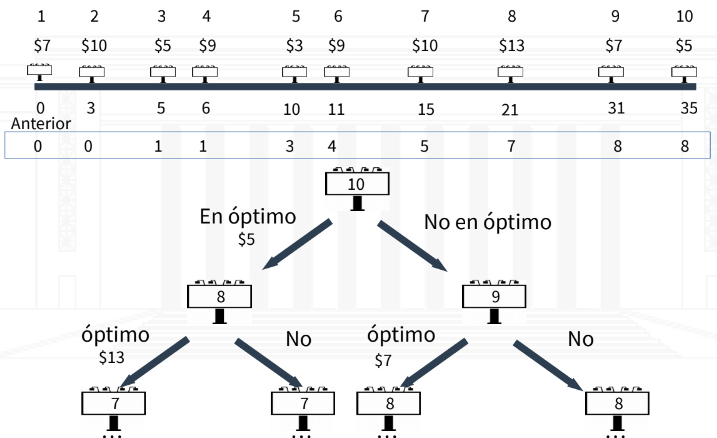
\includegraphics[scale=0.4]{imagenes/dinamico-ruta-arbol.png}
\end{figure}


Para la solución \textbf{recurrente}, podemos plantear:

\[
    \left\{ \begin{array}{lcc}
        OPT(i) = 0 &   si  & i = 0 \\
        \\ OPT(i) = max\{r_i + OPT(anterior(i)), OPT(i-1) \} &  si & i > 0 \\
        \end{array}
    \right.
\]

El resultado con la máxima ganancia sera: \(OPT(n)\). 

\noindent
\textbf{\underline{SOLUCIÓN ITERATIVA}}

\begin{lstlisting}[language=Python, caption=Solución iterativa]

OPT[0] = 0
OPT[1] = r[1]

Desde i=2 a n

    estaCartel = r[i] + OPT[anterior(i)]
    noEstaCartel = OPT[i-1]

    OPT[i] = max (estaCartel, noEstaCartel)

Retornar OPT[n]
\end{lstlisting}


\noindent
\textbf{\underline{SOLUCIÓN ITERATIVA - CARTELES SELECCIONADOS}}

\begin{lstlisting}[language=Python, caption=Solución iterativa con reconstrucción]

OPT[0] = 0
OPT[1] = r[1]
elegidos[0] = false
elegidos[1] = true

Desde i=2 a n

    estaCartel = r[i] + OPT[anterior(i)]
    noEstaCartel = OPT[i-1]

    Si estaCartel>noEstaCartel 
        elegido[i] = true
    sino
        elegido[i] = false

    OPT[i] = max (estaCartel, noEstaCartel)

Retornar OPT[n]
\end{lstlisting}


La complejidad temportal es \(O(n)\) ya que solo hago sumas y comparaciones. La complejidad espacial
es \(O(n)\) porque se almacenan los \(n\) óptimos en un array.

\noindent
\textbf{\underline{SOLUCIÓN ITERATIVA - RECONSTRUIR}}

\begin{lstlisting}[language=Python, caption=Solución iterativa]

i = n

Mientras i>0
    si elegido[i]
        Imprimir i
        i = anterior[i]
    sino 
        i = i-1

Retornar OPT[n]
\end{lstlisting}


La complejidad temportal es \(O(n)\). La complejidad espacial es \(O(n)\).



\noindent
\textbf{\underline{CALCULO anterior de i}}


Se hace un apareo entre las posiciones del cartel \(x\) y el limite del mismo. 
El objetivo es armar un array de anteriores.

\begin{lstlisting}[language=Python, caption=Solución iterativa]

i=n
j=n-1

Mientras i>1
    Si limite(n) >= posicion(j)
        anterior[i] = j
        i=i-1
    sino
        j=j-1

\end{lstlisting}


\newpage
\subsection{Programación de intervalos ponderados}


\newpage
\subsection{Problema de Knapsack (mochila) }

\newpage
\subsection{Problema de Subset Sum }

Sea un conjunto de \(n\) elementos \(E=\{e_1, e_2, ..., e_n \}\) donde cada elemento \(e_i\) 
cuenta con un peso asociado \(w_i\).

Queremos seleccionar un subset de elementos de E con el mayor peso posible que no supere un 
valor \(W\) de peso máximo.

Para plantear una solución por \textbf{fuerza bruta}, un elemento puede estar o no. O sea que si
tengo \(n\) elementos pueden existir \(2^n\) combinaciones. Entonces la complejidad total esta acotado
por \(O(2^n)\).



\newpage
\subsection{Bellman Ford}

Se extiendo el problema de hallar caminos minimos utilizando \textbf{aristas ponderas negativas}. 
Se puede hayar un camino global que pase por aristas ponderadas negativamente y que sea el optimo, 
en vez de utilizar un algotimo de reedy de \textit{Dijkstra} que para este caso no seria óptimo.

Una solución por \textbf{fuerza bruta} seria, calcular para un grafo poderado \textbf{sin ciclos negativos}:

\begin{itemize}
    \item Todos los costos de los caminos posibles de \(s\) a \(t\) de longitud 1.
    \item Todos los costos de los caminos posibles de \(s\) a \(t\) de longitud 2.
    \item ...
    \item Todos los costos de los caminos posibles de \(s\) a \(t\) de longitud n-1.
\end{itemize}

\textbf{El camino mínimo tendra longitud n-1 como máximo} sin ciclos negativos.

El algoritmo de \textbf{Bellman-Ford} halla el camino mínimo con aristas negativos utilizando programación dinámica.

\underline{ANÁLISIS}

Para llegar desde "s" a un nodo \(n_i\) puede haber utilizado diferntes caminino y longitudes.
Lo puede hacer a travez de sus nodos predecesores \(pre[n_i]\).

Para poder llegar a \(n_i\) en \(j\) pasos, tengo que haber llegado a sus predeceroes en \(j-1\) pasos. 
Asi sucesivamente hasta "s" se puede ir resolviendo \textit{sub casos}.

Definimos \(minPath(n,j)\) al camino mínimo hasta el nodo \(n_i\) con longitud máxima \(j\).

\underline{SOLUCIÓN RECURRENTE}

\begin{align*}
minPath('s', j) &= 0 \\
minPath(n_i, 0) &= +\infty & n_i \neq s \\
minPath(n_i, j) &=min\left\{\begin{array}{ll}
                minPath(n_i, j-1)              \\
                min \{minPath(n_x, j-1) + w(n_x, n_i)\}          
        \end{array}\right. & n_x \in pred(n_i)
\end{align*}

\begin{itemize}
    \item El camino mínimo a 's' para cualquier longitud es siempre 0.
    \item El camino mínimo a \(n_i\) al comienzo es infinito.
    \item TODO
\end{itemize}

\underline{SOLUCIÓN ITERATIVA}

Definimos a \(OPT[l][v]\) como el camino mínimo de "s" al nodo \(n\) con longitud\(l\)

El nodo "s" se encuentra en v=0
El nodo "t" se encuentra en v=n

\begin{lstlisting}[language=Python, caption=Algoritmo de requeridos con cupos]
    Desde l=0 a n-1
        OPT[l][0] = 0
    Desde v=0 a n-1
        OPT[0][v] = +infinito


    Desde l=1 a n-1   // max longitud del camino
        Desde v=1 a n // nodo
            OPT[l][v] = OPT[l-1][v]
            Por cada p predecesor de v
                si OPT[l][v] > OPT[l-1][p] + w(p,v)
                    OPT[l][v] = OPT[l-1][p] + w(p,v)
                   
    retornar OPT[n-1, n]
\end{lstlisting}

La complejidad del primer loop esta acotado por n. La segunda parte se ejecuta m veces por cada predecesor.
O sea es \(O(m*n)\)

La complejidad espacial es m*n porque la matriz ocupa n*m

\underline{RECONSTRUIR LAS ELECCIONES}

Agregar un nodo predecesor y almacenar en la posición \(i\) cual fue el predecesor del nodo.

\textit{¿Que pasa si hay un ciclo negativo?}

Si en una iteración despues de haber llegado a la longitud maxima, cambia el minimo de al menos un nodo, entonces el grafo \textit{tiene ciclos negativos}.

\newpage
\subsection{Problema de Maximo subarreglo}

Se necesita calcular un subconjunto \textit{contiguo de elementos} \(S\) 
tal que la suma de los valores sea la máxima posible. 

El maximo subvector que termina en el elemento \(i\), esta relacionado con el máximo
subvector que termina en el elemento \(i-1\).

\underline{SOLUCIÓN RECURRENTE}

\begin{align*}
    MAX(1) &= v[1] \\
    MAX(i) &= max\{MAX(i-1), 0\} + v[i]
\end{align*}
    

\underline{SOLUCIÓN ITERATIVA}

\begin{lstlisting}[language=Python, caption=Solución iterativa]

    MaximoGlobal = v[1]
    MaximoLocal = v[1]
    IdxFinMaximo = 1

    Desde i=2 a n
        MaximoLocal = max(MaximoLocal, 0) + v[i]

        si MaximoLocal > MaximoGlobal
            MaximoGlobal = MaximoLocal 
            IdxFinMaximo = i

    Retornar MaximoGlobal

\end{lstlisting}

\newpage
\subsection{Problema de cuadrados minimos}

Dado un conjunto de puntos \(P={(x_1,y_1),(x_2,y_2),...,(x_n,y_n)}\), con \(x_1<x_2<\cdots<x_n\). 
Usamos \(p_i\) para indicar un punto \((x_i, y_i)\). 

Queremos aproximimar mediante segmentos los puntos de \(P\) minimizando el error comentido. 
Los sementos se forman mediante \textit{rectas de aproximación} hallando \(a\) y \(b\). 
El calculo del error cometido se obtiene sumando las distancias de los puntos a las rectas. 

Se agrega un parametro de penalización \(C>0\) por cada segmento que se agrega.
\begin{itemize}
    \item A mayor "C" entonces: menos segmentos
    \item A menor "C" entonces: menos error
\end{itemize}

Al analizar una solución por \textbf{fuerza bruta} se obtiene una complejidad de \(O(2^{n*n})\).

\underline{SOLUCIÓN RECURRENTE}

Como no conocemos cual es el ultimo segmento, se elige el último segmento como aquel que \textbf{minimice el error general}.  
O sea que queremos minimizar el error del segmento, mas la constante \(c\) 
mas el error conocido en el \textit{subproblema que contiene los puntos de segmentemos anteriores} 
sea el minimo entre todos los posibles.


\begin{align*}
    OPT(i) &= min_{1 \leq x \leq i} (e_{x,i} + C + OPT(x-1)) \\ 
    OPT(0) &= 0
\end{align*}
    
\noindent
\underline{SOLUCIÓN ITERATIVA}

\begin{lstlisting}[language=Python, caption=Solución iterativa]
    OPT[0] = 0

    Para todo para i,j con i <= j
        Calcular e[i][j]

    Desde j=1 a n
        OPTIMO[j] = +infinito
    
        Desde i=1 a n
            segmento = e[i][j] + C + OPT[i-1]

            si OPTIMO[j] > segmento 
                OPTIMO[j] = segmento

    Retornar OPT[n]

\end{lstlisting}

Analizando la \textbf{complejidad temporal}, el calculo del optimo es \(O(n)\), pero se calculan \(n\) óptimos,
Por lo tanto esta partes es \(O(n^2)\).

Pero como en la primer se itera sobre todos los pares posibles es \(O(n)\). Y como el calculo del error
es \(O(n)\), la primer interación termina siendo \(O(n^3)\), y este le gana a \(O(n^2)\).

La complejidad total es \(O(n^3)\).

Para el calculo de la \textbf{complejidad espacial}, los errores se almacenan en \(O(n^2)\), mientras que 
los óptimos en \(O(n)\). Por lo tanto la complejidad espacial total es de \(O(n^2)\).

\newpage
\subsection{Problema del viajante}

Sea un conjunto de \(n\) ciudades "C", un conjunto de rutas de costo de tránsito, existe una ruta 
que une cada par de ciudades.

Queremos obtener el circuito de menor costo que inicie y finalice en una ciudad y
que pase por el resto de las ciudades \textit{una y solo una} vez

Mediante \textbf{fuerza bruta} tenemos que calcular todos los ciclos posibles, y por lo tanto
existen \((n-1)!\) ciclos de longitud \(n-1\). 
Luego por cada ciclo calculamos su costo y nos quedamos con el mínimo. Por lo tanto la complejidad total es \(O(n!)\).

Mediante el \textbf{algoritmo Belman-Held-Karp} lo resuelvo utilizando programación dinamica.
Se puede decomponer como el mínimo entre los subproblemas menores con \((n-1)!\) hojas.

\noindent
\underline{SOLUCIÓN RECURRENTE}

Dado \(S\) un subconjunto de ciudades e \(i\) la ciudad donde estoy parado. \textbf{start} es la ciudad de partida.
La siguiente es la ecución de recurrencia:

\begin{align*}
    OPT(i, \{S\}) &= min_{j \in \{S\}} (w(i,j) + OPT(j, \{S-j\})) \\ 
    OPT(i, \emptyset) &= w(i, start)
\end{align*}

\begin{itemize}
    \item El optimo i con el subconjuto s va a ser igual al minimo de los subproblemas que son elegir alguna de las ciudades que estan en s. 
          Sumando el peso de i a j mas el optimo de partir de j hacia el resto de las ciudades (s-j).
    \item En el caso base, ya no quedan ciudades para visitas, entonces solo queda sumar el peso de ir de \(i\) a la ciudad de inicio \textit{Start}.
\end{itemize}
    
\noindent
\underline{SOLUCIÓN ITERATIVA}
Llamamos a \(C\) al conjunto de todas las ciudades, 1 es la ciudad inicial, y el resto de las ciudades
estan numeradas de 2 a n.


\begin{lstlisting}[language=Python, caption=Solución iterativa]

    Desde i=2 a n
        OPT[i][0] = W[i][1]
    
    Desde k=1 a n-2
        Para todo subset S de C-{1} de tamanio k
            Para cada elemento i de S
                OPT[i, S-{i}] = +infinito

                Por cada elemento j de S - {i}
                    r=OPT[j, S-{i,j}] + w[j][i]

                    si (r<OPT[i, S-{i}])
                        OPT[i, S-{i}] = r

    
    CamininoMinimo=+infinito
    Desde j=2 a n
        ciclo = OPT[i, S-{1, i}] + w[1, i]
        Si (CamininoMinimo>ciclo)
            CamininoMinimo = ciclo
    
    Retornar CamininoMinimo

\end{lstlisting}

\begin{itemize}
    \item La primer iteración se cargan los casos bases para las \(n\) ciudades.
    \item Despues desarrollamos los subproblemas, primero iteramos las ciudades que quedan por visitar
    \item Luego generamos las variantes de subset y por cada uno calculo el minimo y 
    utilizo los subproblemas de tamaño menor, ver cual de todos es el minimo.
\end{itemize}

La complejidad total es \(O(n^2 2^n)\)

\newpage
\section{Redes de flujo}

\subsection{Conceptos}

Se trata de problemas de flujos de trafico en redes. 
Por ejemplo, tubos de gas, autopistas, rutas de aviones, redes electricas.

Definiciones:
\begin{itemize}
    \item Los \textbf{ejes} transportan algun tipo de flujo
    \item Los \textbf{vértices} actúan como conmutador de tráfico entre los diferentes ejes.
    \item Capacidad: cantidada máxima que un eje puede transportar.
    \item Fuente: Vértices que generan tráfico saliente.
    \item Sumidero:Vértice que absorbe tráfico entrante.
    \item Flujo: Cantidad transportada por eje.
\end{itemize}

Sea \(G=(V,E)\) un grafo dirigido, para todo \(e \in E\) llamamos \(C_e \geq 0\) (valor entero) a su capacidad.
Existe un único \(s \in V\) llamado fuente (source). O sea no tiene ejes entrantes.
Existe un único \(t \in V\) llamado sumidero (sink). O sea no tiene ejes salientes.
El resto de los vertices son internos como si fueran conmutadores de fuentes.

\noindent
\textbf{\underline{DEFINICION DE FLUJO}}
El flujo \(s-t\) es una funcion \(f\) que mapea cada \(e\) a un número real no negativo,
\(f: E \mapsto R^+\). Un flujo tiene las siguientes caracteristicas:

\begin{itemize}
    \item (Condición de capacidad) Para cada \(e \in E\), tenemos que \(0 \leq f(e) \leq C_e\).
    \item (Condición de conversación) Para cada nodo \(v\) que no sean \(s\) y \(t\) , tenemos que:
    \[
        \sum_{e into v} f(e)  = \sum_{e out of v} f(e) 
    \]
\end{itemize}

\noindent
\textbf{\underline{PROBLEMA DE FLUJO MAXIMO}}

Definimos \textbf{corte de grafo} como: 

Dos cortes diferentes, tienen capacidades de transporte maxima diferentes.


\newpage
\subsection{Algoritmo Ford-Fulkerson}

Calcula el maximo flujo a travez de una red.

\noindent
\underline{\textbf{Grafo residual}}

Dado un red de flujo \(G\) y un flujo \(f\) en \(G\), 
\textbf{definimos el grafo residual \(G_f\) (de \(G\) con respecto a \(f\))} a:

\begin{itemize}
    \item Los mismos vértices de G,
    \item \textbf{Ejes hacia adelante}: Para cada \(e=(u,v) \in E\) en el que \(f(e) < C_e\). 
    Lo incluimos en \(G_f\) con capacidad \(C_e-f(e)\) [\textbf{capacidad residual} de flujo].
    \item \textbf{Ejes hacia atras}: Para casa \(e=(u,v) \in E\) en el que \(f(e) > 0\). 
    Incluimos \(e'=(v,u)\) con capacidad \(f(e)\).
\end{itemize}

\noindent
\underline{\textbf{Cuello de botella}}

Sea \(P\) un \textbf{camino simple} \(s-t\) en \(G_f\), o sea que \(P\) no visita más de una vez el mismo vértice.

Difinimos \textbf{bottleneck(P,f)} a la \underline{capacidad residual mínima} de cualquier eje de P con repecto al flujo \(f\).

\begin{figure}[h!]
    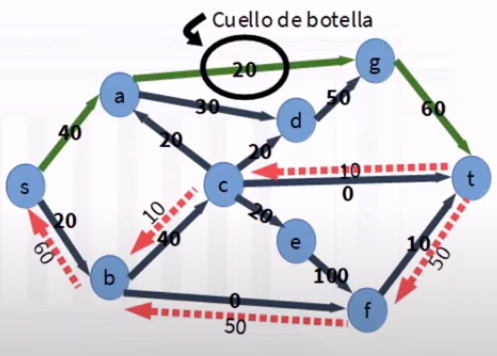
\includegraphics[width=\linewidth]{imagenes/cuello-de-botella.png}
\end{figure}

Lo máximo que se puede transportar es 20, para que no deje cumplir la condición de capacidad.

\begin{quote}
    \textit{Con el grafo residual, podemos redireccionar el flujo en el camino original para aumentar el flujo total de la red.}
\end{quote}

Tambien nos ayuda a saber cuanto flujo se esta trasportando por ese eje.

Llamamos \(P\) al camino de aumento (\textbf{augmenting path}):

\begin{itemize}
    \item \(P\) es una caminio simple que va de \(s\) a \(t\) en \(G_f\).
    \item \(P\) no visita el mismo nodo mas de una vez.
\end{itemize}
 
Ahora definimos la operación \textbf{augment(f,P)} el cual cede un nuevo flujo \(f'\) en e\(G\)

\begin{lstlisting}[language=Python, caption=Operación de augment]
augment(f, p)
    Sea b = bottleneck(P, f)
    Para cada eje e=(u, v) perteneciente a P
        Si e=(u,v) eje hacia adelante
            f(e) += b en G
        sino si es eje para atras 
            e' = (v,u)
            f(e') -=b en G   
    Retornar f
\end{lstlisting}


\begin{figure}[h!]
    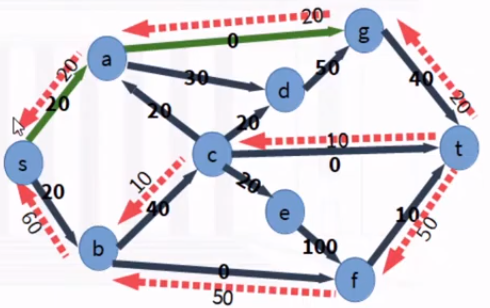
\includegraphics[width=\linewidth]{imagenes/camino-aumento.png}
\end{figure}

\textit{¿Es valido el nuevo flujo?}PENDIENTE

Con el grafo residual y el camino de aumento definimos el \textit{pseudocódigo de Ford-Fulkerson}.


\begin{lstlisting}[language=Python, caption=Operación de augment]
Max-Flow
    Inicialmente  f(e)=0 para todo 'e' en G

    Mientras haya un camino s-t en Gf

        Sea P un caminio s-t simple en Gf
        f' = augment(f,P)

        Actualizar f para ser f'
        Actualizar Gf para ser Gf'


    Retornar f
\end{lstlisting}

La \textbf{complejidad} es \(O(|E|*C)\) donde \(|E|\) es la cantidad de ejes y C es la suma de todas
las \(C_e\) de los ejes que salen de la fuente.


\textit{¿Es óptimo?}PENDIENTE

\begin{quote}
    \textbf{El flujo retornado por el algoritmo Ford-Fulkerson es el flujo máximo}
\end{quote}

Ademas podemos mediante BFS en \(G_f\) construir el corte mínimo s-t (A,B) obteniendo A y por diferencia B.

Consideraciones si las capacidades no son enteras:
\begin{itemize}
    \item Si son racionales, multiplicar por minimo comun multiplo
    \item Si son irracionales, \textit{no esta asegurado que el algoritmo termine}.
\end{itemize}

\subsection{Variante: Circulación con demanda}

Cada nodo pueder ser productor o consumir de flujo. O un nodo que no es consumidor ni productor de flujo.

\newpage
\subsection{Bipartite Matching Problem}

Llamamos un grafo bipartito a \(G=(V,E)\) un \textit{grafo no dirigido}, puede particionarse en 
como \(V=X \cup Y\), con la propiedad de que cada eje \(e \in E\) se conecta en una punta con
un nodo en \(X\) y la otra punta un nodo en \(Y\). Un \textit{matching M} en \(G\) es un subconjunto
de ejes \(M \subseteq E\) tal que cada nodo aparece en al menos un eje en \(M\).
Se necesita encontrar el set \(M\) de mayor tamaño posible. O sea la mayor cantidad de parejas.


Resolvemos el matching utilizando el problema de flujo máximo.
Construimos una red de flujo \(G'\) como la siguiente imagen. Pasamos todos los ejes a ejes dirigidos de
\(X\) a \(Y\). Luego agregamos el nodo \(s\) y un eje \((s,x)\) desde \(s\) a cada nodo en \(X\). 
Tambien agregamos el nodo \(t\) y un eje \((y,t)\) desde cada nodo en \(Y\) a \(t\).
Finalmente, le damos una capacidad de \(1\) a cada eje en \(G'\)

\begin{figure}[h!]
    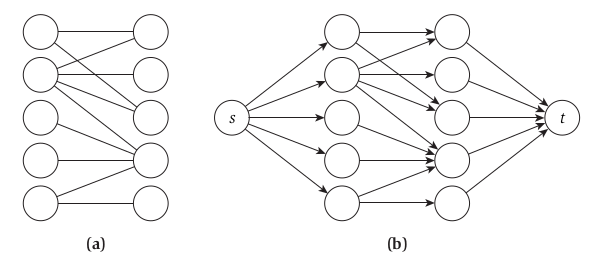
\includegraphics[width=\linewidth]{imagenes/bipartito-redes-flujo.png}
\end{figure}

Resolvemos el problema de red de flujo máximo con \(G'\). Obtenemos el flujo máximo \(s-t\). Entonces
\textit{El valor del flujo total es igual al tamaño del matiching máximo.}

\textbf{Analisis} Pendiente

\newpage
\subsection{Diseño de encuentas}

Considere el problema de una compañia que vende \(k\) productos y que tiene una base de datos con el 
historias de las compras de todos sus clientes. La compañia desea enviar encuestas con preguntas
personalizadas a un grupo particular de \(n\) clientes, para determinar que productos la gente 
prefiere sobre el total.

Lineamientos para la encuesta:
\begin{itemize}
    \item Cada cliente recibira preguntas acerca de cierto subconjunto de productos.
    \item Un cliente solo puede contestar sobre los productos que él o ella haya comprado.
    \item Cada cliente sera preguntado sobre un número de productos entre \(c_i\) y\(c'_i\) 
    \item Cada producto debe tener entre \(p_j\) y \(p'_j\) preguntas de clientes distintos.
\end{itemize}

El problema de diseño de encuentas toma como input un \textit{grafo bipartito} \(G\) cuyos nodos son 
clientes y productos, y hay un eje entre un cliente \(i\) y un producto \(j\) si el cliente compro el producto \(j\).
Mas aún, por cada cliente \(i=1,2,...,n\) tenemos la limitante de \(c_i \leq c'_i\) en el numero de productos en el que un 
cliente puede constestar; por cada producto \(j=1,...,k\), tenemos la limitante \(p_j \leq p'_j\) en el 
número de cliente distintos que se pueden consultar por cada producto.

\begin{figure}[h!]
    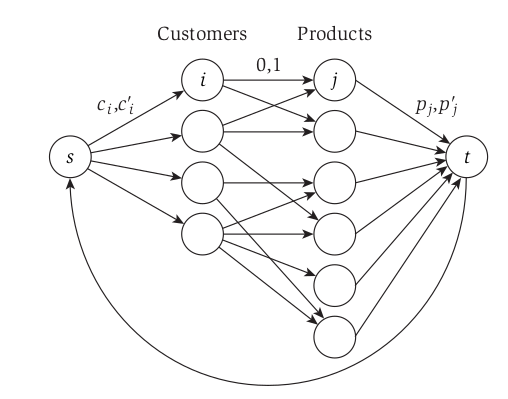
\includegraphics[width=\linewidth]{imagenes/grafo-encuesta.png}
\end{figure}

El problema se resuelve reduciendo este a un problema de red de flujo en \(G'\) con demanda y un limite inferior. 

Para obtener un grafo \(G'\) de \(G\), necesitamos:
\begin{itemize}
    \item Orientar los ejes de \(G\) desde los clientes a los productos.
    \item Agregar un nodo ficticio \(s\) con los ejes \((s,i)\) por cada cliente \(i=1,...,n\).
    \item Agragar un nodo ficticio \(t\) con los ejes \((j,t)\) por cada producto \(j=1,...,k\).
\end{itemize}

La circulacion en la red, corresponde con la manera en la que se tienen que realizar las preguntas.

Se debe pasar de un problema de circulación con \textit{demanda y limite inferior} a un problema
de circulación con demanda y luego a un problema de flujo máximo. Finalmente se resuelve con Ford-Fulkerson.

Una vez obtenido el flujo máximo:

\begin{itemize}
    \item El flujo que va de \((t,s)\) corresponde al número total de preguntas a realizar.
    \item El flujo en los ejes \((s,i)\) es el número de productos que deben contener el cuestionario para cada cliente \(i\).
    \item El flujo en los ejes \((j,t)\) corresponde con él numero de clientes que deben ser preguntados para el producto \(j\).
    \item Por ultimo, aquellos ejes \((i,j)\) con flujo 1, corresponden a preguntar al cliente \(i\) sobre el producto \(j\).
\end{itemize}

\newpage
\subsection{Problema de Selección de proyectos}

Dado un conjunto \(P\) de proyectos para seleccionar y cada proyecto \(i \in P\) tiene
asociado una ganancia \(p_i\), el cual puede ser \textit{positivo} como \textit{negativo}.
Algunos proyectos son requisitos de otros proyectos, y modelaremos esta relación mediante un \textit{grafo
dirigido sin ciclos} \(G=(P,E)\). Los nodos de \(G\) son los proyectos y hay un eje \((i,j)\) para indicar
que un proyecto \(i\) puede ser seleccionado solo si el proyecto \(j\) es tambien seleccionado.
Un proyecto \(i\) pude tener muchos prerequisitos, y puede haber muchos proyectos \(j\) que pueden
ser parte de esos prerequisitos. Un conjunto de proyecto de \(A \subseteq P\) es \textit{viable} si los 
prerequisitos de cada proyecto de \(A\) tambien pertenecen a \(A\):
\begin{quote}
    Por cada \(i \in A\) y cada eje \((i,j) \in E\), tenemos que \(j \in A\)
\end{quote}
Estos prerequisitos vendrian a ser las \textit{restricciones de precedencia}. La ganancia del conjunto de proyectos
se define como:

\[
    profit(A) = \sum_{i\in A} p_i 
\]

El \textit{problema de selección de proyectos} seleccionar el conjunto de proyectos viables con la maxima ganancia.


\newpage
\section{Problemas NP}

\subsection{Clasificación}

\subsubsection{Clase P}

La clase \(P\) consiste en aquellos problemas que pueden resolverse en tiempo polinomial (eficientemente).

Un algoritmo A resuelve \textbf{eficientemente} un problema \(S\) si para toda instancia \(I\) de \(S\),
encuentra la solución en tiempo polinomico, entonces existe una constante \(k / A = O(n^k)\) 
y donde \(n\) es el tamaño de la entrada del problema. 
Ejemplo, Gale Shapley resuelve el problema de "Stable Marriage Problem" en \(O(n^2)\)

Se conoce como \(P\) al conjunto de problemas de decisión para los que existe un algoritmo que lo resuelva en
\textit{forma eficiente}.

Un algoritmo B \textbf{certifica eficientemente} un problema de decisión \(S\)  si para toda instancia \(I\) de \(S\),
dado un certificado \(t\) que contiene evidencia de la solución \(s(i)\) es \textit{"Si"}, 
entonces existe una constante \(k / B = O(n^k)\). 

O sea que el algoritmo B va a recibir dos parametros, la instancia \(I\) y el certificado \(T\).  
Responde si o no. Por ejemplo, en el problema de la moneda, seria las cantidades de monedas a dar, 
y certificado seria la solución conocida. Para validar, se ejecuta el algoritmo de certificación
con el certificado \(T\).


\subsubsection{Clase NP}

Se conoce como \(NP\) al conjunto de problemas de decisión para los que existe un algoritmo
que lo verifique (certifique) en tiempo polinomial (eficientemente).

¿\(P \subseteq NP\)?. Si el problema \(Q \in P\), existe un algoritmo \( A = O(n^k)\) que lo resuelve. Y podemos definir como:

\begin{lstlisting}[language=Python, caption=Algoritmo B]

    B(I, t)
        s = A(I)
        Si s == t
            retornar "si"
        retornar "no"

\end{lstlisting}

Que certifica el problema \(Q\) y lo hace en tiempo polinomial. Entonce se cumple:

\[
    Q \in P \implies Q \in NP
\]

¿\(NP \subseteq P\)?. Es un problema sin resolver.


\subsection{Reducciones}

Reducir un problema a otro conocido.

\begin{figure}[h!]
    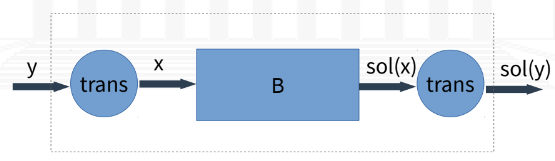
\includegraphics[width=\linewidth]{imagenes/reduccion.png}
\end{figure}

Una reducción polinomial corresponde a una reducción en la que ambas transformaciones se realizan en tiempo polinonimial.

Sean X, Y problemas, diremos \(Y \leq_p X\), se lee Y es polinomialmente reducible (en tiempo) a "X"

Si podemos transformar cualquier instancia de \(Y\) en una instancia de \(X\) en tiempo polinomico (tractable).

Para \textbf{comparar problemas} con reducciones, sean \(X, Y\) problemas, si \(Y \leq_p X\), diremos que 
el problema \(X\) es al menos tan dificil que el problema \(Y\)

Para \textbf{acotar un problema} a la clase \(P\). 
\begin{itemize}
    \item Sean \(X,Y\) problemas si \(X \in P\) y \(Y \leq_p X\) 
    entonces \(Y \in P\), porque \(X\) es igual de complicado que \(Y\). Ejemplo:
    \begin{gather*}
        MAXMATCHING \leq_p MAXFLOW \\
        MAXFLOW \in P \implies MAXMATCHING \in "P"    
    \end{gather*}
    
    \item Sean \(X,Y\) problemas si \(Y \notin P\) y \(Y \leq_p X\) 
    entonces \(X \notin P\), porque \(X\) es igual de complicado que \(Y\).
    
\end{itemize}

Las siguientes son propiedades de reducciones:

\begin{itemize}
    \item \textit{Equivalencia}: Sean \(X,Y\) problemas si \(Y \leq_p X\) y \(X \leq_p Y\) 
    entonces \(X\) e \(Y\) tiene la misma complejidad.
    \item \textit{Transitividad}: Si \(Z \leq_p Y\) y \(Y \leq_p X\) 
    entonces \(Z \leq_p X\)
\end{itemize}


\subsection{Clase NP completo}

\subsubsection{Problema de satisfabilidad booleana - SAT}
Dado un conjunto de variable booleanas que definen una expresión booleana, determinar si existe una
asignación de valores de las variables, tal que el resultado de la expresión es "TRUE".

Sea una instancia \(I\) del problema \textbf{SAT} \(\in NP\) y un certificado que corresponde a un valor
de asignación de cada variable.

Podemos certificar en tiempo polinomial si esa asignación de variables producen un resultado "TRUE".

El \textbf{teorema de Cook-Levin} dice, sea \(X \in NP\) entonces \(X \leq_p\) Boolean satisfability problem (SAT). 
O sea, \textbf{que todo problema perteneciente a NP es a lo sumo tan complejo de resolver que SAT}.
 
\textbf{NP-HARD}: Sea un problema \(X\) tal que para todo problema \(Y \in NP\) y \(Y \leq_p X\), entonces \(X \in NP-HARD\).
\textbf{X es al menos igual de dificil que cualquier problema NP}.

\textbf{NP-Complete}: Sea un problema \(X\) tal que para todo problema \(X \in\)NP-HARD y \(Y \in \) NP, entonces \(X \in NP-C\).
\textbf{X es uno de los problemas mas dificiles dentro de NP}.

\underline{Ejemplo de uso}, para cada problema de \(X \in NP\) que analiza Richard Carp, toma un problema 
demostrado como NP-C y lo reduce a \(X\), con esto \(X\) pasa a ser un problema \textbf{NP-C}.

\textbf{Probar que un problema} es \textit{NP-C}. Sea el problema \(X\) de decisión. Probamos:

\begin{itemize}
    \item Probar que \(X \in NP\), definiendo un certificado eficiente:
    \item Probar que \(X \in NP\)-HARD, dado un problema \(Y \in NP\)-C, 
    reducir polinomialmente \(Y\) a \(X\). Eligiendo el problema \(Y\) correcto para reducir, 
    podemos obtener \(Y \leq_p X\) y agregar a \(X\) en la clasificación de los problemas \textit{NP-C}.
\end{itemize}


\subsection{Problema de conjunto independiente}

Sea un grafo \(G=(V,E)\), un valor \(K\), determinar si existe un conjunto independiente de nodos 
de como mucho tamaño k.

Definimos un conjunto de nodos \(C \subseteq V\) es independiente si no existe \(a,b \in C\) tal que existe eje \((a,b) \in E\) 
y el \textbf{tamaño del conjunto independiente} corresponde con la cantidad de nodos dentro del conjunto C.

\begin{figure}[h!]
    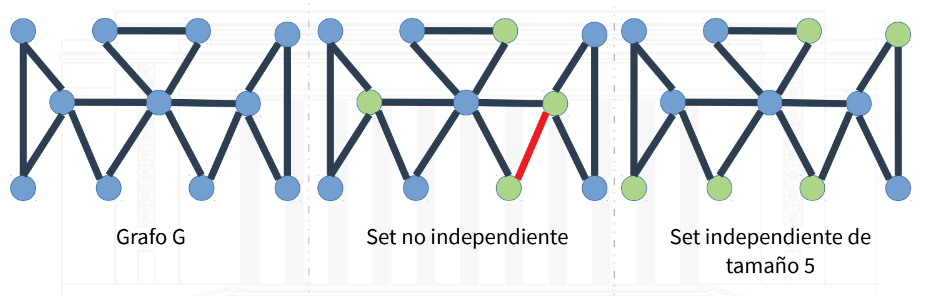
\includegraphics[width=\linewidth]{imagenes/conjunto-independiente.png}
\end{figure}

Dado un grafo \(G=(V,E)\) con tamaño \(k\) de conjunto y un certificado \(T\) igual 
al subconjunto de nodos. Si se puede verificar en tiempo polinomial con \(|T| = K\) que:
\[
    \forall a,b \in T, !\exists (a,b) \in E \implies INDEPENDENTSET \in NP    
\]

\subsubsection{3-SAT}
Es una variante de SAT donde cualquier instancia de SAT se puede reducir polinomialmente a 3SAT:

\[
    SAT \leq_p 3SAT \implies 3SAT \in NPComplete
\]

Dado \(X={x_1,...,x_n}\) conjunto de \(n\) variables booleanas = \(\{0,1\}\) y 
\(k\) \textit{clausulas} booleanas \(T_i=(t_{i1} \lor t_{i2} \lor t_{i3} )\) 
con cada \(t_{ij} \in X \cup \overline{X} \cup {1}\). Entonces debemos 
\textbf{determinar si existe asignación de variables} tal que \(T_1 \land T_2 \land ... \land T_k = 1\)

\newpage
\subsubsection{Reducción de 3-SAT a INDEPENDENT-SET}
Por cada \textit{clausula} \(T_i=(t_{i1} \lor t_{i2} \lor t_{i3} )\) \textbf{vamos a generar tres vertices entre si}.
Y por cada \(t_{ij}=x_a,t_{kl}=\overline{x_a} \), crear un eje entre \(t_{ij}\) y \(t_{kl}\).

\begin{figure}[h!]
    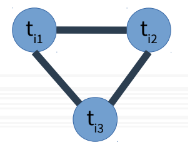
\includegraphics[scale=0.4]{imagenes/reduccion-3sat.png}
\end{figure}

\textbf{El grafo resultante }\(G\) corresponde a una instancia del problema \textit{INDEPENDENT-SET} 
con k=numeros de clausulas en la expresión. Ejemplo, sea la expresión:

\(E=(x_1 \lor x_2 \lor x_3) \land (\overline{x_1} \lor \overline{x_2} \lor \overline{x_4}) 
    \land (\overline{x_2} \lor \overline{x_3} \lor x_4) 
    \land (\overline{x_1} \lor \overline{x_2} \lor x_3)\)

Reducimos polinomialmente y resuelvo:
\begin{figure}[h!]
    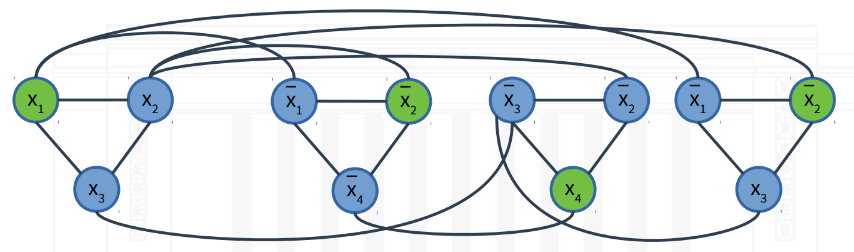
\includegraphics[scale=0.4]{imagenes/ejemplo-reduccion-3sat.png}
\end{figure}

Entonces, luego resuelvo 3SAT con \(x_1 = 1\), \(\overline{x_2} = 1 \implies x_2=0\), 
\(x_4=1\) y elijo \(x_3=0\) porque en este caso es indistinto.

Por lo tanto, como INDEPENDENT-SET \(\in NP\) y \(3SAT \leq_p INDEPENDENTSET\) NP.

Entonces INDEPENDENT-SET \(\in NPComplete\)

\newpage
\subsection{Problema de cobertura de vertices}
Sea un grafo \(G=(V,E)\) diremos que existe un conjunto \(S \subseteq V\) es una cobertura de vétices si:
\[
    \forall \;eje\; e \in E=(u,v), u\in S \;\; y/o \;\; v \in S
\]
Donde \(u\) y/ó \(v\) pertenecen al conjunto \(S\).

El \textbf{problema de decisión} sera que dado un grafo \(G=(V,E)\), determinar si existe una conbertura
de vértices (VERTEX-COVER) de tamaño al menos \(k\). 
\textbf{El problema de optimización busca el subconjunto de menor tamaño}.


\begin{figure}[h!]
    \begin{center} 
    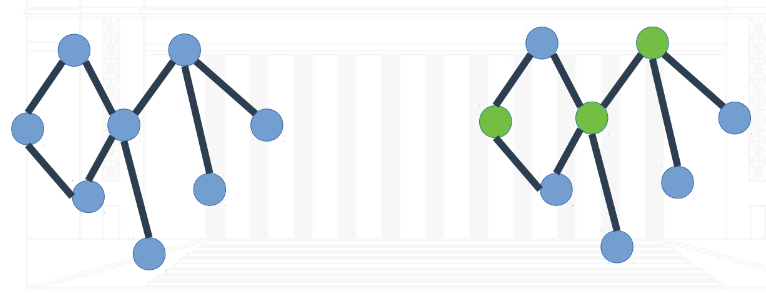
\includegraphics[width=\linewidth]{imagenes/ejemplo-cobertura-v-k3.png}
    \caption{\small \sl Ejemplo de conbertura de vertices de k=3.\label{fig:Stupendous}} 
    \end{center}
\end{figure}

Para ver si VERTEX-COVER pertenece a un \textbf{problema NP}, verificamos de la siguiente manera: 

Sea un grafo \(G=(V,E)\) y un certificado \(T\) como un conjunto de nodos de \(V\) que forman el cubrimiento. 
Verificamos que:
\[
    \forall \;eje\; e \in E=(u,v), \; si \; u\in T \;\; o \;\; v \in T \implies O(V*E)
\]
observamos si uno de estos vertices pertenece al certificado y lo podemos ver en tiempo polinomial de \(O(V*E)\) y si ademas \(|T|=k\), 
entonces el certificado nos da la respuesta con tamaño k, y por lo tanto \textbf{VERTEX-COVER} \(\in\) \textbf{"NP"}

Para ver si VERTEX-COVER pertenece a un \textbf{problema NP-Completo}, utilizaremos INDEPENDENT-SET.

\newpage
\subsection{Problema de cobertura de conjunto}

Sea un conjunto \(U\) de \(n\) elementos. Una colección \(S_1,...,S_m\) de subconjuntos de U. 
Problema de decisión: ¿Existe una colección de como mucho \(k\) de los subconjuntos cuya unión es igual a U?

La idea es probar que SET-COVER es NP-COMPLETO. Sea U un conjunto de elementos, 
K tamaño buscado, los subset \(S_1,...,Sm\) y un \(T\) certificado con los indices de los subconjuntos del conjunto.

Verificamos que \(|T|=k\) para todo elemento en \(U\), si existen en algunos de los subconjuntos de \(T\). 
Por lo tanto se puede hace en tiempo polinomial y se puede afirmar que \textbf{SET-COVER es "NP"}.

Luego elegimos un problema que previamente se haya demostrado que es NP-Completo. Para esto vamos a usar VERTEX-COVER.
Vamos a intentar demostrar que VERTEX-COVER \(\leq_p\) SET-COVER. El algoritmo de reducción sera:

\newpage
Para la \textbf{reducción de VERTEX-COVER a SET-COVER}, partimos de \(G=(V,E)\) y \(k\). Queremos que todos los ejes
queden cubiertos y construimos un conjunto de elemtentos U=E. Por cada vertice \(v \in V\), 
creamos un subconjunto \(S_v\) con todos los ejes incidentes a el, y mantenemos en \(k\) la cantidad
de subconjuntos a buscar para cubrir U. Toda esta transformación se puede hacer en tiempo polinomial.

Si encontramos el subconjunto, eso nos dira que vertices seleccionar.

\begin{figure}[h!]
    \begin{center} 
    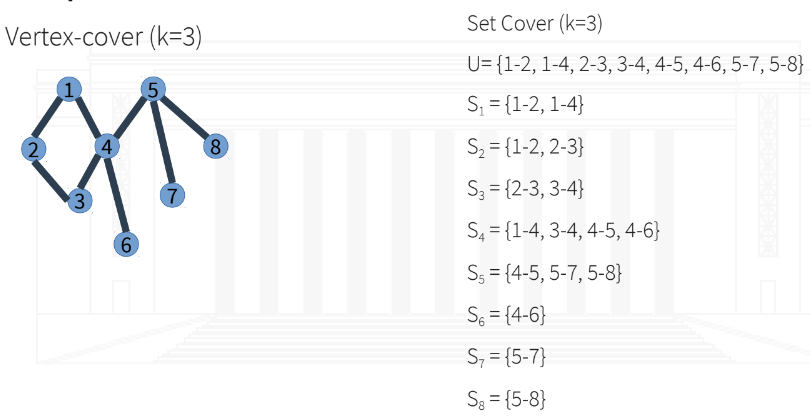
\includegraphics[width=\linewidth]{imagenes/ejemplo-set-cover.png}
    \caption{\small \sl Ejemplo de reducción de VERTEX-COVER a SET-COVER.\label{fig:Stupendous}} 
    \end{center}
\end{figure}

Si se resuelve SET-COVER, se obtiene los subconjuntos que corresponden a los nodos resultantes en el 
problema de VERTEX-COVER.

Resumiendo, demostramos que SET-COVER es NP-COMPLETO, porque reducimos VERTEX-COVER a SET-COVER en tiempo
polinomial, y si resolvemos cualquier instancia de set-cover, podemos resolver cualquier instancia
de vertex-cover.

\newpage
\subsection{Problema 3 Dimensional Matching}

Dado 3 conjuntos disjuntos \(X, Y, Z\) de tamaño \(n\) 
cada uno y un conjunto \(C \subset X \times Y \times Z\) de trip\(X, Y, Z\)las ordenadas. Determinar si existe
un subset de \(n\) triplas ene \(C\) tal que cada elemento de \(X \cup Y \cup Z\) sea contenido
exactamente en una de esas triplas.

\begin{figure}[h!]
    \begin{center} 
    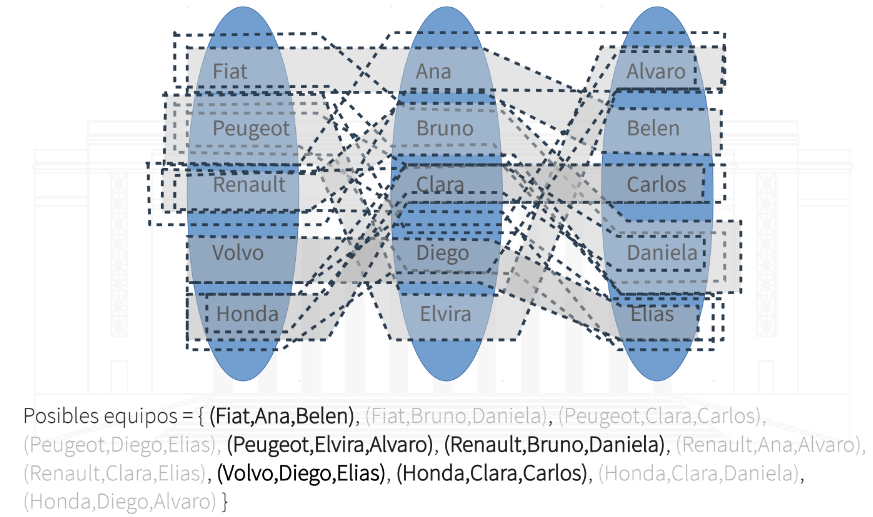
\includegraphics[width=\linewidth]{imagenes/ejemplo-3DM.png}
    \caption{\small \sl Ejemplo de uso de 3DM.\label{fig:ejm3dm}} 
    \end{center}
\end{figure}

Para verificar que 3DM pertence a NP, dado 3 conjuntos disjuntos \(X, Y, Z\), \(C=(x,y,z)\) 
conjunto de triplas y un certificado \(T\), de triplas con un subconjunto de C.

Podemos certificar en tiempo polinomial que todo elemento en X, Y y Z, \underline{se encuentra 1 
y solo 1 vez en algun} \(T_i\). Y si \(|T|=n\), entonces:
\[
    3DM \in NP
\] 

Ahora queremos probar que 3DM pertenece a los problemas NP-HARD. Probamos que \(3SAT \leq_p 3DM\).

Sea \(I\) instancia de 3SAT con \(n\) variables \(x_1,...,x_n\) y \(k\) clausulas \(c_1,...,c_k\), 
reducimos en tiempo polinomial la instancia \(I\) a un problema 3DM.

PENDIENTE DE REDUCCION Y DEMOSTRACION.

\subsection{Ciclo Hamiltoneano}
Sea un grafo G=(V,E) dirigido definimos un ciclo C en G como hamiltoneano si visita cada vértice
1 y solo 1 vez. Es un recorrido que inicia y finaliza en el mismo vertices.

El problema de decisión sera HAM-CYCLE, sea G=(V,E) grafo dirigido, ¿existe un ciclo hamiltoneano?


\begin{figure}[h!]
    \begin{center} 
    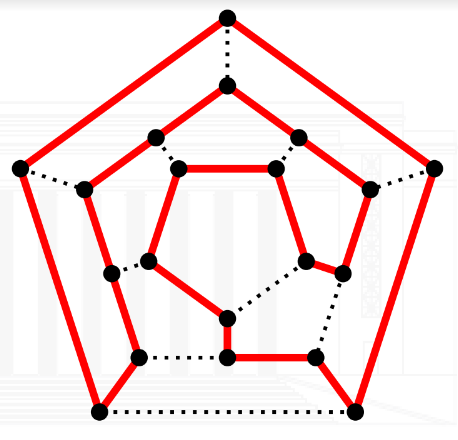
\includegraphics[scale=0.3]{imagenes/ejemplo-ciclo-hamilton.png}
    \caption{\small \sl Ejemplo de un ciclo de hamilton.\label{fig:hamilton-ej}} 
    \end{center}
\end{figure}

Para saber si el HAM-CYCLE pertenece a NP, dado un grafo G=(V,E) 
y un certificado \(T = \{t_0,...,t_{|v|}\}\) lista ordena de vertices.
Puedo verificar en tiempo polinomial los siguientes puntos:

\begin{enumerate}
    \item La cantidad nodos en T es igual a la cantidad de vertices en V. \(|T|=|V|\) y \(t_0=t_|M|\).
    \item Todos los vértices de V estan en T.
    \item Para todo par de vertices \(t_i, t_{i+1} \in T\) existe un eje direccionado \((t_i, t_{i+1}) \in E\) que los une. 
    O sea seguimos el camino ordenado de nodos.
\end{enumerate}

Por lo tanto podemos afirmar que \textbf{HAM-CYCLE}\(\in NP\).

NP C - PENDIENTE

\section{Algoritmos Randomizados}

Un algoritmo randomizado es aquel que resuelve un problema P utilizando 
como parametro extra una cadena aleatoria "\(r\)". Las decisiones de ejecución
se realizan teniendo en cuenta la lectura de la cedena aleatoria.

\textbf{Clase de complejidad RP}: Se conoce como "RP" o "R" a aquellos problemas de decisión
para los que existe un programa "M" randomizado que se ejecuta en tiempo polinomial. Y que para 
toda instancia \(I\) del problema:
\begin{itemize}
    \item Si la instancia \(I\) debe tener como resultado "Si", entonces:
     \[
         Probabilidad(M(I,r)="Si")\geq 1/2
     \] 
    \item Si la instancia \(I\) debe tener como resultado "No" (no debe tener falsos positivos), entonces:
    \[
        Probabilidad(M(I,r)="No") = 0
    \] 
    
\end{itemize}

\textbf{Clase de complejidad co-RP}: Se conoce como "RP" o "R" a aquellos problemas de decisión
para los que existe un programa "M" randomizado que se ejecuta en tiempo polinomial. Y que para 
toda instancia \(I\) del problema:
\begin{itemize}
    \item Si la instancia \(I\) debe tener como resultado "Si" (no debe tener falsos negativos), entonces:
     \[
         Probabilidad(M(I,r)="No") = 0
     \] 
    \item Si la instancia \(I\) debe tener como resultado "No", entonces:
    \[
        Probabilidad(M(I,r)="No") \geq 1/2
    \]
\end{itemize}

\textbf{Clase de complejidad ZPP}: Se conoce como \textit{zero-error probabilistic P} (ZPP) a aquellos
problemas de decisión que pertenecen a "RP" y "co-RP". Implica que para toda instancia I del problema
podemos ejecutar el algoritmo en RP y co-RP, entonces en tiempo polinomial tendremos 3 respuestas posibles:
"Si", "No" y "No es posible".

La repetición de un número no determinado de ejecuciones nos asegura obtener el resultado correcto.
Este tipo de clase de complejidad corresponde a los algoritmos de \textbf{Las Vegas}, en la intersección RP \(\cap\) co-CP.


\textbf{Clase de complejidad BPP}: Se conoce como \textit{bounded-error probabilistic P} (BPP) a aquellos problemas de decisión
para los que existe un programa "M" randomizado que se ejecuta en tiempo polinomial. Y que para 
toda instancia \(I\) del problema:
\begin{itemize}
    \item Si la instancia \(I\) debe tener como resultado "Si", entonces:
     \[
         Probabilidad(M(I,r)="Si") \geq 2/3
     \] 
    \item Si la instancia \(I\) debe tener como resultado "No", entonces:
    \[
        Probabilidad(M(I,r)="Si") \leq 1/3
    \]
\end{itemize}

No podemos estar seguros. Si el resultado es correcto, podemos afirmarlo con "alta probabilidad".
Este tipo de clase de complejidad corresponde a los algoritmos de \textbf{Monte Carlo}.

\begin{figure}[h!]
    \begin{center} 
    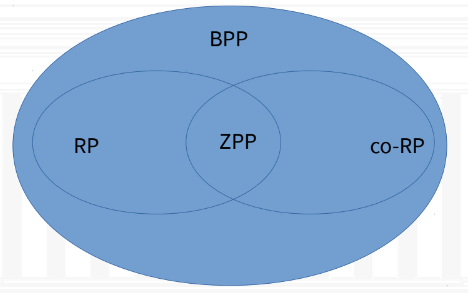
\includegraphics[scale=0.3]{imagenes/relacion-rp-p-zpp-bpp.png}
    \caption{\small \sl Relación entre clases.\label{fig:hamilton-ej}} 
    \end{center}
\end{figure}

\newpage
\subsection{Mezcla aleatoria}

Sea un conjunto A de \(n\) elementos que queremos generar un listado de A ordenado aleatoriamente.
Mezclar conjuntos se utilizan en \textit{juegos de azar, reproducción de musica aleatoria, modelos estadisticos 
simulaciones, pruebas de complejidad algoritmica y otros mas}.

\textbf{Permutación por ordenamientos}: 
Para cada \(i\) elemento en A, generaremos un numero \(p_i\) aleatorio como su clave.
Utilizando \(p_i\) para cada elemento \(a_i\) como "clave", ordenaremos "A". Podemos elegir 
cualquier metodo de ordenamiento como caja negra para resolverlo. O sea ordenamos basandonos
en la clave aleatoria que generamos para cada elemento.


\begin{lstlisting}[language=Python, caption=Algoritmo de permutación por odenamiento]
Sea A[1..n] conjunto a ordenar
Sea P[1..n] vector numerico // vector de prioridades.

Desde j=1...n
    P[j] = random_value(1...x)

Ordenamos A utilizando P como clave

Retornar A
\end{lstlisting}

Este algoritmo tiene un problema y es que si se generan claves repetidas, en metodos de 
ordenamientos como los estables, no se realizara la permutación y de esta forma no se podra 
obtener una permutación aleatoria uniforme (en terminos de probabilidad). 

Para disminuir la posibilidad de claves repetidas, tenemos que tomar las siguientes acciones:

\begin{enumerate}
    \item Podemos establecer un valor de X muy alto. \(X >>> n \) (Por ejemplo \(n^5\)).
    \item Se puede agregar un registro de claves utilizadas y volver a seleccionar otra clave 
            si surge una ya utilizada. En el peor de los casos, se puede obtener siempre la misma
            clave y por consiguiente entrar en un loop infinito, si se elige mal el valor de \(x\).
\end{enumerate}

La complejidad temporal es \(O(n log(n))\) por que la generación de claves es \(O(n)\) y el ordenamiento
es \(O(n log(n))\) por lo que mandan el ordenamiento. La complejidad espacial es \(O(n)\).

Según el análisis de uniformidad cualquier permutación tiene probabilidad \(1/n!\).
Por lo tanto este método genera una \textit{permutación aleatoria uniforme}.

\textbf{Algoritmo de mezcla de Fisher-yates}: Tambien se conoce como "barajado de sombrero".
Se introducen todos los números en un sombrero, se agita el contenido(se mezclan) y se van sacando
de a uno y se listan el mismo orden en el que se sacan hasta que no queden ninguno.

La descripción algoritmica es, para cada elemento A[i], generamos un calor \(x\) al azar entre \(i\) y \(n\). 
Luego intercambiamos A[i] con A[x].

\begin{lstlisting}[language=Python, caption=Algoritmo de Fisher-yates]
Sea A[1..n] conjunto a ordenar

Desde i=1...n
    intercambiar A[i] con A[random_value(i...n)]

Retornar A
\end{lstlisting}    

Según el análisis de uniformidad cualquier permutación tiene probabilidad \(1/n!\).
Por lo tanto este método genera una \textit{permutación aleatoria uniforme}.

La complejidad temporal es O(n) porque tenemos \(n\) interaciones, y dentro de cada interación
tenemos un intercambio que es O(1) y un ramdom que tambien es O(1). La complejidad espacial 
es O(1) porque todo el algoritmo se puede hacer sobre el mismo vector.

Ejemplo con \(A=\{a_1,a_2,a_3,a_4\}\):
\begin{figure}[h!]
    \begin{center} 
    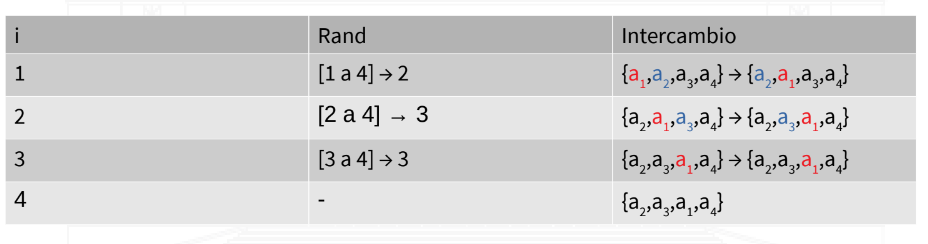
\includegraphics[scale=0.3]{imagenes/ejemplo-mezcla-aleatoria.png}
    \caption{\small \sl Ejemplo de mezcla de Fisher-yates} 
    \end{center}
\end{figure}

\subsection{Problema de K conectividad de en un grafo}

Sea \(G=(V,E)\) grafo conexo y no dirigido, deseamos saber ¿cuantos ejes se pueden remover antes 
que G deje de ser conexo?. Se espera encontrar la minima cantidad de ejes para que se un grafo conexo.

\begin{figure}[h!]
    \begin{center} 
    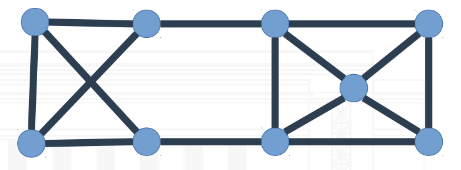
\includegraphics[scale=0.5]{imagenes/ejemplo-k-conectividad.png}
    \caption{\small \sl Ejemplo de k conectividad} 
    \end{center}
\end{figure}

Analizamos el problema y lo podemos pensar como encontrar el corte global mínimo del grafo si
analizamos toda posible subdivisión A-B del grafo en 2 conjuntos disjuntos. En cada 
subdivisión contamos la cantidad de ejes entre conjuntos y tomamos la subdivisión con menor 
de ejes. Resolverlo por fuerza bruta, tendria una complejidad exponencial.

\begin{figure}[h!]
    \begin{center} 
    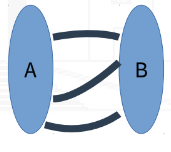
\includegraphics[scale=0.5]{imagenes/ejemplo-subdivicion.png}
    \caption{\small \sl Ejemplo de k conectividad} 
    \end{center}
\end{figure}

Para solver el problema, vamos a realizar una reducción al problema de flujos:

\begin{enumerate}
    \item Por cada eje \(e=(u,v)\) creamos 2 ejes dirigidos (u,v) y (v,u), les asignamos una capacidad de 1.
    \item Por cada combinación posible de dos nodos, etiquetamos como s y t respectivamente y resolvermos \textit{"MAX-FLOW MIN-CUT"}.
    \item El menor de los cortes mínimos corresponde al valor de la K-conectividad del eje del grafo.
\end{enumerate}

\begin{figure}[h!]
    \begin{center} 
    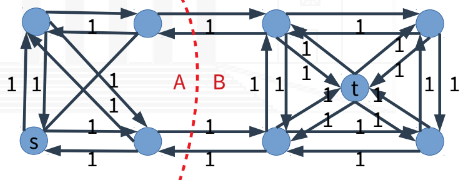
\includegraphics[scale=0.5]{imagenes/ejemplo-k-mincut.png}
    \caption{\small \sl Ejemplo de k conectividad} 
    \end{center}
\end{figure}

La complejidad temporal va a ser \(O(n^5)\) ya que por una lado, vamos a repetir el problema de flujo maximo en \(O(|V|^2)\)
y por el otro en el peor de los casos, si usamos ford-fulkenson la complejidad sera \(O(|V|^3)\).

\textbf{Algoritmo de Karger}:


\newpage
\section{Algoritmos de aproximación}

\subsection{Problema del balanceo de carga}

Dado un conjunto de maquinas \(M_1,M_2,..,M_m\), un conjunto de \(n\) tareas donde cada tarea \(j\)
requiere \(T_j\) de tiempo de procesamiento. El objetivo es asignar las tareas a las maquinas
de tal forma que la carga quede balanceada (El tiempo asignado a cada maquina sea lo mas parejo posible).



\end{document}




